%\documentclass{acm_proc_article-sp}

%\usepackage{url}
%\usepackage{graphicx}
%\usepackage{wrapfig}
%\usepackage{fancybox}
%%\usepackage{todonotes}
%\usepackage[disable]{todonotes}

%\usepackage{listings}

%\newtheorem{req}{Requirement}
%\newtheorem{definition}{Definition}
%\newtheorem{ex}{Example}

\newcommand{\code}[1]{\texttt{#1}}
%\newcommand{\eg}{e.g.,~}
%\newcommand{\ie}{i.e.,~}
%\newcommand{\Ie}{That is,~}
%\newcommand{\Eg}{For example,~}
% \newcommand{\url}[1]{\href{#1}{#1}}


\newcommand{\searchword}{family-friendly}
% \newcommand{\url}[1]{\href{#1}{#1}}

\newcommand{\placeholder}{\code{urn:placeholder}}
\newcommand{\placeholderB}{\code{urn:placeholder2}}

\hyphenation{me-thods}
\hyphenation{ori-gi-na-ting}
\hyphenation{sear-ching}
\hyphenation{func-tio-na-li-ties}


%\begin{document}
\lstset{language=Java}
\chapter{A Service-oriented Search Framework for Full Text, Geospatial and Semantic Search}
%
% You need the command \numberofauthors to handle the 'placement
% and alignment' of the authors beneath the title.
%
% For aesthetic reasons, we recommend 'three authors at a time'
% i.e. three 'name/affiliation blocks' be placed beneath the title.
%
% NOTE: You are NOT restricted in how many 'rows' of
% "name/affiliations" may appear. We just ask that you restrict
% the number of 'columns' to three.
%
% Because of the available 'opening page real-estate'
% we ask you to refrain from putting more than six authors
% (two rows with three columns) beneath the article title.
% More than six makes the first-page appear very cluttered indeed.
%
% Use the \alignauthor commands to handle the names
% and affiliations for an 'aesthetic maximum' of six authors.
% Add names, affiliations, addresses for
% the seventh etc. author(s) as the argument for the
% \additionalauthors command.
% These 'additional authors' will be output/set for you
% without further effort on your part as the last section in
% the body of your article BEFORE References or any Appendices.

%\numberofauthors{6} %  in this sample file, there are a *total*
% of EIGHT authors. SIX appear on the 'first-page' (for formatting
% reasons) and the remaining two appear in the \additionalauthors section.
%
%\newcommand{\unisterAddr}{
%       \affaddr{R\&D, Unister GmbH}\\
%    \affaddr{Barfussgaesschen 11}\\
%    \affaddr{Leipzig (Germany)}\\
%}
%\author{
% You can go ahead and credit any number of authors here,
% e.g. one 'row of three' or two rows (consisting of one row of three
% and a second row of one, two or three).
%
% The command \alignauthor (no curly braces needed) should
% precede each author name, affiliation/snail-mail address and
% e-mail address. Additionally, tag each line of
% affiliation/address with \affaddr, and tag the
% e-mail address with \email.
%
% 1st. author
%\alignauthor
%Andreas Both\\
%       \unisterAddr
%       \email{andreas.both@unister.de}
%% 2nd. author
%\alignauthor
%Axel-Cyrille Ngonga Ngomo\\
%       \affaddr{Universit\"at Leipzig, IFI/AKSW }\\
%%       \affaddr{Leipzig }\\
%       \affaddr{Leipzig (Germany)}\\
%       \email{ngonga@informatik.uni-leipzig.de}
% 3rd. author
%\alignauthor 
%Ricardo Usbeck\\
%       \affaddr{Universit\"at Leipzig, IFI/AKSW}\\
%       \affaddr{Unister GmbH, Leipzig}\\
%       \email{usbeck@informatik.\\uni-leipzig.de}
%\and  % use '\and' if you need 'another row' of author names
% 4th. author
%\alignauthor        
%Denis Lukovnikov\\
%       \affaddr{Universit\"at Leipzig, IFI/AKSW }\\
%       \affaddr{Leipzig }\\
%       \affaddr{Leipzig (Germany)}\\
%       \email{lukovnikov@informatik.uni-leipzig.de}
% 5th. author
%\alignauthor 
%Christiane Lemke\\
%       \unisterAddr
%       \email{christiane.lemke@unister.de}
% 6th. author
%\alignauthor 
%Maximilian Speicher\\
%       \affaddr{TU Chemnitz, VSR}\\
%       \affaddr{Unister GmbH, Leipzig}\\
%       \email{speim@hrz.tu-chemnitz.de}
  % use '\and' if you need 'another row' of author names
% 5th. author
%\alignauthor Sean Fogarty\\
%       \affaddr{NASA Ames Research Center}\\
%       \affaddr{Moffett Field}\\
%       \affaddr{California 94035}\\
%       \email{fogartys@amesres.org}
% 6th. author
%\alignauthor Charles Palmer\\
%       \affaddr{Palmer Research Laboratories}\\
%       \affaddr{8600 Datapoint Drive}\\
%       \affaddr{San Antonio, Texas 78229}\\
%       \email{cpalmer@prl.com}
%} % author
%\date{15 June 2014}
% Just remember to make sure that the TOTAL number of authors
% is the number that will appear on the first page PLUS the
% number that will appear in the \additionalauthors section.

%\maketitle
%\begin{abstract}
Over the last decade, a growing importance of search engines could be observed. 
An increasing amount of knowledge is exposed and connected within the Linked Open Data Cloud, which raises users' expectations to be able to search for any information that is directly or indirectly contained. 
However, diverse data types require tailored search functionalit\-ies\----such as semantic, geospatial and full text search. 

Hence, using only one data management system will not provide the required functionality at the expected level.
In this paper, we will describe search services that provide specific search functionality via a generalized interface inspired by RDF. 
In addition, we introduce an application layer on top of these services that enables to query them in a unified way. 
This allows for the implementation of a distributed search that leverages the identification of the optimal search service for each query and subquery.
This is achieved by connecting powerful tools like \textit{Openlink Virtuoso}, \textit{ElasticSearch} and \textit{PostGIS} within a single framework. 
%Finally, we will isolate the performance challenges.
%\end{abstract}
% A category with the (minimum) three required fields
%\category{TODO}{TODO}{TODO}
%A category including the fourth, optional field follows...
%\category{TODO}{TODO}{TODO}[TODO]

%\terms{Distributed Search, Semantic Web, Information Retrieval}

% \keywords{ACM proceedings, \LaTeX, text tagging} % NOT required for Proceedings

\section{Introduction}

%\todo[inline]{find a new wording for federated, Vorschlag: hybride suche, dann kann man das PhD Syposiums Paper zitieren mit :'The search functionality to be developed in this thesis is going to be hybrid,i.e., simultaneously performing a full text,e.g., Lucene-based5 , and an entity search.' und schreiben, dass man es hier erweitern möchte}
Over the last two decades, the content of the World Wide Web has grown to an enormous collection of webpages. 
In addition, users have shifted their preference from desktop to Web applications.
This is primarily driven by growing technical capabilities of Web browsers as well as the demand for exploiting the knowledge available on the Web.
Particularly, large Web application providers---including Google, Bing and \mbox{Yahoo}!---promise that any kind of information will be made available through simple search queries. 

In recent years, a very large number of datasets have been published based on Semantic Web standards.
More than 61 trillion triples\footnote{\url{http://stats.lod2.eu/}, retrieved June 16, 2014.} are available through the \emph{Linked Open Data} (LOD) cloud by now.
Instead of publishing text documents containing unstructured information, the new paradigms demand information which are structured by standards like the \textit{Resource Description Framework} (RDF)\footnote{\url{http://www.w3.org/TR/rdf11-concepts/}}.
RDF can be used for for publishing logical properties like \code{typeOf} relations (\eg Germany is of the type \code{country}), standard type properties (\eg the number of people living on a square kilometer within Germany: \code{229}) or complex data types such as geospatial coordinates (\eg \code{POINT(13.3833, 52.5167)} in the case of Germany).
Since this data is published in a standardized format (\ie RDF), it can be read and processed by machines.
This provides opportunities for creating novel industrial applications. 

The trend just described leads to a situation in which a vast amount of unstructured information is available on the Web next to a large amount of structured data accessible for automatic processing by machines.
While the latter data representation enables direct access of annotated knowledge and a derivation of insights, the knowledge of the textual representations (mostly HTML documents) is not directly accessible in an easy way. 
Thus, information retrieval methods are needed in a preprocessing step to compute semantic information which can be annotated within the (HTML) document.

In the course of the current developments, users will tend to reject search solutions based on the knowledge originating from one data representation only. 
On the one hand, Google's Web search\footnote{\url{http://www.google.com}} demonstrates the advantages of searching huge collections of textual documents. 
On the other hand, applications like Wolfram Alpha\footnote{\url{http://www.wolframalpha.com/}} and Apple's Siri\footnote{\url{https://www.apple.com/de/ios/siri/}} present the advantages of knowledge-driven search functionalities.

\todo[inline]{Below is the first time we're mentioning e-commerce. Should we not introduce the application area earlier? CL}
Thus, a search infrastructure is required, which is capable of integrating the functionalities of textual search with search methods working on top of annotated semantics. 
User demands in the context of e-commerce are particularly driven by queries for products (\ie the type of the subject of interest), such as ``hotel'', ``flight'' or ``winter holiday''.
Additionally, properties can express the requirements posed on the subject of interest. 
Three different types have to be considered in this case:
\begin{itemize}
\item logical properties, \eg ``has wifi'', ``suitable for vegetarians'';
\item geospatial properties, \eg ``north of London'', ``close to a beach'';
\item properties driven by textual information, \eg ``pool for children''\footnote{We assume that such properties are not directly modeled in the underlying structured knowledge base.} or a part of the name of the searched entity (like ``Kempinski'').
\end{itemize}

All three types of queries are well supported by specific instances of data stores:

\begin{itemize}
\item searches for logical properties are implemented by triple stores, \eg the Openlink Virtuoso Server~\cite{erling2009rdf};
\item searches for geospatial properties are supported by data\-base\ management systems with extensions for geo\-gra\-phic information system (GIS), \eg PostGIS~\cite{obe2011postgis}, an open source software program that adds support for geographic objects to the PostgreSQL object-relational database~\cite{momjian2001postgresql};
\item searches within text documents are supported by index-based data stores, \eg the scalable search solution ElasticSearch~\cite{kuc2013elasticsearch} based on Apache Lucene~\cite{hatcher2004lucene}.
\end{itemize}

\todo[inline]{AnBo: Add more about SOA.}

In this paper, we will present an architectural layer on top of these well-known search solutions.
%This architecture provides an integrational concept atop of well-known functionality.
In particular, we will take care of preserving their scalability aspects, like the search on large sets of text documents.
A data representation close to RDF will be used within our architecture. 
However, there is no need for using a particular data store for semantic data (\ie mostly a triple store) since our approach is agnostic with respect to the backends used. %used data stores.
Our main contribution is an engineering approach for creating a scalable search solution capable of conducting semantic search with geospatial aspects as well as information retrieval from text documents. The benefits of the different search systems are combined and integrated in order to better deliver on the expectations of the users. 
%Hence, our main contribution is an engineering approach for creating a scalable search functionality that is capable of conducting semantic search (including geospatial aspects) as well as information retrieval from text documents.
 
The rest of the paper is organized as follows. Section \ref{chafedsearch:sec:related} addresses related work while Section \ref{chafedsearch:sec:architecture} describes general requirements for our approach as well as its architecture.
Subsequently, we present our approach to search query representation in Section~\ref{chafedsearch:sec:searchqueryanalysis} and introduce our approach to interpreting search queries in Section~\ref{chafedsearch:sec:queryinterpretation}.
Section~\ref{chafedsearch:sec:federated} describes our federated search architecture, before giving concluding remarks in Section~\ref{chafedsearch:sec:conclusion}.
%\todo[inline]{AnBo: Check outline.}


\section{Related Work}
\label{chafedsearch:sec:related}
Our approach is related to the research area of search over Linked Data and thus to keyword search and question answering (QA) over Linked Data.
% Therefore, we call it Semantic Entity Search. 
% Question Answering attempts to find an answer to user queries posed in natural language. 
Several systems have been developed for the latter task.
One of the first systems was AquaLog~\cite{aqualog}, an ontology-driven QA system for the Semantic Web. 
Aqualog uses linguistic analysis to transform the input query to a set of query-triples. 
Then, these query triples are interpreted using lexical resources and the given ontology. 
The interpreted query-triples are sent to an inference engine to find the answer.
One major drawback of AquaLog is that it is limited to one ontology at a time.
To address this and other drawbacks of AquaLog, PowerAqua~\cite{poweraqua} was developed.
PowerAqua follows an approach similar to that of AquaLog, reusing AquaLog's linguistic analysis.
However, PowerAqua performs more advanced query-triple interpretation using different ontologies simultaneously.


Treo~\cite{treo} is a method for querying Linked Data that relies on spreading activation.
First, pivot entities in the query are identified.
Then, from the dependency structure of the input sentence, Treo constructs a Partially Ordered Dependency Structure (PODS).
The PODS is used to resolve the query in the spreading activation search step where semantic relatedness scores are used to rank candidates and subsequently spread activation.
Pythia~\cite{pythia} is a more recent QA system.
It uses lexica that define mappings between a syntactic and a semantic representation of an expression.
With these lexica, Pythia also introduces a distinction between ontology-dependent and ontology-independent lexica. 
Whereas the former depends on the verbalizations of entities from some ontology, the latter describe ontology-independent expressions (determiners, question words,...).
The sentence is parsed using such lexica and the resulting semantic representation is translated to a formal query.
Building upon Pythia's dichotomy between ontology-dependent and -independent lexical entries, TBSL~\cite{tbsl} presents a tem\-plate-based QA approach. 
This approach consists of 3 steps. First, SPARQL query templates are generated by using do\-main-specific and generic language resources.
The template slots are filled by using a combination of resource lookup and natural-language patterns extracted using the BOA framework~\cite{BOA}. The resulting SPARQL queries are finally scored and the best query (i.e., the highest ranking query that returns a non-empty result set) is selected and returned. 
More recently, several novel systems have participated in the QALD-3 challenge on QA over Linked Data~\cite{qald3}.  
CASIA~\cite{casia} (the currently best-performing system on the QALD-3 benchmark dataset) relies on a three-step approach resembling AquaLog's architecture.
During the first step, the question type is determined and text triples are constructed from the dependency parse tree of the question sentence. 
In the second step, RDF resources which match phrases from the text triples are detected. 
CASIA uses relation extraction patterns from PATTY~\cite{patty} to map text fragments to properties and classes.
In the final step, a SPARQL query is generated based on the question type and the RDF resources detected in the input question.
CASIA achieves an F-score of $0.36$ on the QALD-3 benchmark.

Approaches on keyword-based querying of the Web of Data include SINA~\cite{sina} and the work of Tran et al.~\cite{tran}.
SINA~\cite{sina} aims at answering a keyword question using diverse datasets.
First, simultaneous disambiguation and segmentation is performed using Hidden Markov Models (HMM) and the Hyper\-link-Induced Topic Search (HITS) algorithm.
The found resources are used to construct an Incomplete Query Graph (IQG) consisting of disjoint sub-graphs.
To build the federated SPARQL query that retrieves the results, the IQG's are connected using a Minimum Spanning Tree approach inspired by Prim's algorithm.
The work of Tran et al.~\cite{tran} tackles the problem of keyword search over RDF data.
More specifically, the work of Tran et al. is concerned with mapping keywords to a list of ranked conjunctive queries, with a special focus on efficient inference of implied connections.
To accomplish this, a top-k algorithm is proposed that computes the best query interpretations of the keyword query using bidirectional graph exploration.
The interpretations are then scored and mapped to conjunctive queries.
The performance of the proposed top-k approach is evaluated 
on DBLP.

Generic frameworks for searching over RDF data have been suggested in the past.
For example, the OKBQA framework\footnote{\url{http://www.okbqa.org}} presents a modular architecture for search over structured and unstructured sources.
This architecture is yet not fully instantiated and it is thus difficult to compare with our approach.

Usbeck~\cite{DBLP:conf/esws/Usbeck14} presents a generic architecture for hybrid search using a holistic framework comprising information extraction methods for unstructured~\cite{AGDISTIS} and semi-structured data sources.%~\cite{REX}.
Afterwards, the framework combines the underlying heterogeneous data stores to answer keyword and natural language queries via transforming each query into generic SPARQL queries returning only the highest ranked results.%~\cite{HAWK}.
\todo[inline]{Final: Add ESWC 2014 and ISWC 2014 papers}

In contrast to the state of the art, we propose a generic framework which integrates state of the art approaches for search over both Linked Data, unstructured data and arbitrary APIs.

In~\cite{fedsearch}\ a federated SPARQL search engine--FedSearch-- is presented, which presents a hybrid combination of SPARQL and full-text search tackling data heterogeneity and lacking statistical data.
Since SPARQL lacks full-text search support the authors propose a triple-store-independent way of querying different RDF stores such as OWLIM, Virtuoso and LuceneSail.
Their vendor independent approach of keyword query search pattern is evaluated next to several optimizations against two benchmarks showing superior performs against other state-of-the-art systems.

Meta-search engines (\eg~\cite{liebel2004harvester,gulli2005building}) are a different approach for taking advantage of the power of different search services.
However, meta-search engines do not re-use intermediate results to refine parts of the search query, at the most they improve the representation by re-ranking or clustering the summarized search results (\eg~\cite{carpineto10metasearchclustering}).

Service-oriented architecture (SOA)~\cite{Gartner96,OASIS06} can be seen as an architectural pattern providing the needed tools for organizing the communication between distributed (software) components~\cite{bell2009soa}.
The SOA manifesto\footnote{http://soa-manifesto.org/} prioritizes intrinsic interoperability over custom integration, shared services over specific-purpose implementations and flexibility over optimization. 
Its main purpose is providing an infrastructure for connecting loosely coupled components by defining processes using dynamic component discovery and registration~\cite{erl2008soa}.

Thus, the goals of SOAs are close to the ones of Linked Data.
In contrast, SOA is interface-driven not data-driven like Linked Data. 
In particular, it is not connected to SPARQL or RDF.
However, the concepts can be combined aiming for the best of both worlds, e.g., as~\cite{yu2011linked} has shown for the e-learning domain.


\section{High-Level Architecture and General Requirements}\label{chafedsearch:sec:architecture}
\begin{figure}[t]
\centering
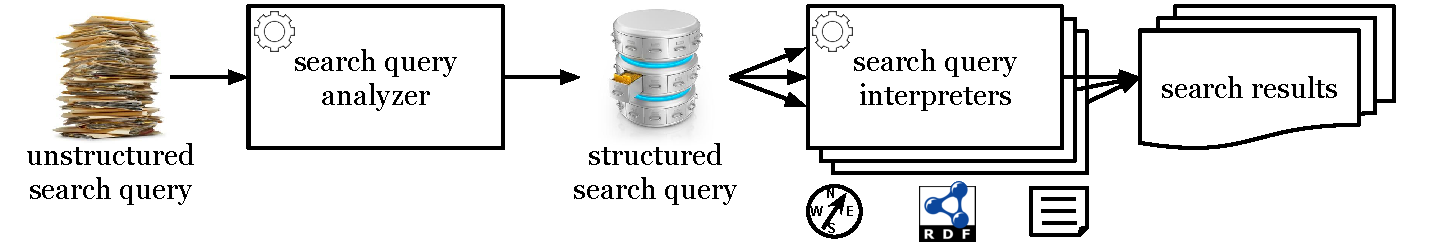
\includegraphics[width=\textwidth]{part_03/SEMANTiCS_architecture/highlevelarchitecture2}
\caption{High-level architecture of our distributed search framework.}
\label{fig:highlevelarchitecture}
\end{figure}


The concept of a service-oriented search framework poses several specific requirements that have to be met to rea\-lize a corresponding architecture.
They will be described in the following.
\todo[inline]{citation?}
\todo[inline]{or at least a note we came up with this ourselves? - CL\\will be at the last paragraph of the related work -- AnBo}
First of all, the framework has to ensure the integrability of the various intended search functionalities, which is derived from the properties of (extensible) service-oriented architectures:
%Derived from the properties of (extensible) service-oriented architectures, a generalized interface needs to enable the integration of various search functionalities.
%\todo[inline]{seems like a repetition to me}
%To ensure this, the following requirement has to be obeyed:
\begin{req}
An interface for search services has to be defined. The definition has to comprise a  summarization of all needed attributes for controlling the execution of (sub)queries.
\end{req}

We focus on a generalized approach, especially w.r.t. the communication across the diverse search services. Thus, we demand:
\begin{req}
The communication with the search services has to be stateless and transparent.
\end{req}
Derived from the required stateless and transparent communication, each search service has to encode all information about itself via its interface ,\ie in the message during the communication\footnote{This requirement is comparable to REStful communication~\cite{richardson2008restful} via the stateless HTTP protocol \url{http://tools.ietf.org/html/rfc7231}.}.
Hence, the information about each search service has be retrieved by querying the implemented interface methods.
%\todo[inline]{I don't get the last two sentences, to which requirement they belong and what they have to do with the next sentences? -CL\\Better? -- AnBo}
However, to provide a structured search query, an analysis of the textual user input is needed, which we consider to be beyond the scope of this paper. 
We will assume the search query is already available in a structured representation (\eg by having used approaches like~\cite{similarity,aqualog,tbsl}).
%For the sake of the limited space, we assume each search query to be already analyzed.
%That is, it was transformed into a structured representation, e.g., by using approaches like~\cite{similarity,aqualog,tbsl}.

\begin{req}\label{req:allrelevantparts}
The search query requires a structured representation which encapsulates information about all relevant parts of the search query. 
\end{req}

Hence, the high-level infrastructure of a federated search requires a two-step process:
\begin{enumerate}
\item search query analyzer
    \begin{itemize}
    \item input: unstructured search query
    \item output: structured search query
    \end{itemize}
\item search query interpreter
    \begin{itemize}
    \item input: structured search query
    \item output: ranked search results 
    \end{itemize}
\end{enumerate}
\todo[inline]{maybe markup structured search query everywhere\\ Why? -- AnBo}
\todo[inline]{Add reference to basic SOA paper at $\ast$ to support the seemingly arbitrary statement. --Max}
A graphical overview of the workflow is shown in Figure~\ref{fig:highlevelarchitecture}. 
To achieve the intended service-oriented architecture, it is crucial to hide the implementation details of the contained search services \cite{erl2008soa}.
As sketched in Figure~\ref{fig:highlevelarchitecture}, the structured search query is the main carrier of information.
Hence, no knowledge about the behavior of a particular search service may be contained in a structured search query, except in the case that it was computed by a search service itself. 
This is because the structured search query has to be independent from the particular implementation of any search service to ensure their exchangeability within the service-oriented architecture.
The following requirement is derived:
\begin{req}\label{req:independence}
The structured search query representation has to be independent from the implementation of any particular search service.
\end{req}

In the following, we will describe the data structure required for the representation of an analyzed search query.


\section{Search Query Representation}\label{chafedsearch:sec:searchqueryanalysis}

Understanding what the user is looking for is the starting point of every information retrieval process.
Yet, in the following section, the focus is not on the analysis of unstructured search queries.
Rather, search query analysis is considered a black box, \ie we focus on the representation of the structured search query after analysis.

%\subsection{Search Query Representation}
%Our representation is close to RDF.
%Hence, the following definition holds:
For our purpose, we build on a search query representation that is close to RDF:
\begin{definition}[RDF triples]
Assume there are pairwise disjoint infinite sets $I$, $B$, and $L$ representing IRIs\footnote{\textit{Internationalized Resource Identifier}, \ie a URI that may contain any Unicode character (cf.~\url{http://tools.ietf.org/html/rfc3987}).}, blank nodes, and RDF literals, respectively. 

A triple $(v_1, v_2, v_3) \in (I \cup B) \times I \times (I \cup B \cup L)$ is called an RDF triple. 
We call $v_1$ the subject, $v_2$ the predicate and $v_3$ the object. 
We denote the union $I \cup B \cup L$ by $T$ called RDF terms.
\end{definition}

However, we need a definition of the target resource.
Therefore, we allow a specific IRI to indicate the target elements, \ie our system performs a pure resource search.
For the sake of simplicity, we denote it as follows:


\todo[inline]{Warum sind es auf einmal urns? --RU}
\begin{definition}[Searched resource]
The place hold\-er for the searched resource is denoted as \placeholder.  
\end{definition}

\todo[inline]{Add example to clarify that \placeholder\ is what we actually search for and thus also acts as the root of the topologically sorted tree mentioned later. --Max}

Obviously, this mechanism can be used for referencing different variables by adding any ID (\eg \placeholderB).

\todo[inline]{The example query does not contain XXX used in its explanation later. Neither does the example in figures 2 and 3 contain the feature family-friendly. -CL}
For example, it is possible to express an actual search query, \eg \texttt{family-friendly hotel in Leipzig} in the following way:
Potential target hotels (\code{urn:id:hotel}) are restricted to those being located in the city center of Leipzig (expressed using the relation \code{urn:rel:cityCenter}).
Furthermore, a target hotel has to be marked (\code{urn:rel:hasFeature}) as family-friendly (\code{urn:id:familyFriendly}) and the description of the hotel has to contain the word \searchword.
The corresponding search query representation is shown in Figure~\ref{fig:ex1}.
\begin{figure}
\begin{center}
\begin{tabular}{llll}
$t_1$ & \placeholder & \code{owl:typeof} & \code{urn:id:hotel} \\
$t_2$ & \placeholder & \code{urn:rel:citycenter} & \code{urn:id:Leipzig} \\
$t_3$ & \placeholder & \code{urn:rel:description} & \placeholderB \\
$t_4$ & \placeholderB & \code{urn:rel:sublabel} & ``\searchword''
\end{tabular}
\end{center}
\caption{Example of a structured search query \texttt{family-friendly hotel in Leipzig} according to our RDF-like representation.}
\label{fig:ex1}
\end{figure}
\newcommand{\sstriplestore}{\code{urn:service:triplestore}}
\newcommand{\ssfulltext}{\code{urn:service:fulltext}}
\newcommand{\ssgeo}{\code{urn:service:gis}}
\begin{figure}[t]
\begin{center}
\begin{tabular}{lllll}
$t_1$ & \placeholder & \code{owl:typeof} & \code{urn:id:hotel} & ({\sstriplestore},250,500) \\
$t_2$ & \placeholder & \code{urn:rel:citycenter} & \code{urn:id:Leipzig} & (\ssgeo,100,400) \\
$t_3$ & \placeholder & \code{urn:rel:description} & \placeholderB & ({\sstriplestore},4000,1000) \\
$t_3$ & \placeholder & \code{urn:rel:description} & \placeholderB & (\ssfulltext,300,200) \\
$t_4$ & \placeholderB & \code{urn:rel:sublabel} & ``\searchword'' & (\ssfulltext,300,200) 
\end{tabular}
\end{center}
	\caption{Example of an annotated search query \texttt{family-friendly hotel in Leipzig}.}
	\label{fig:ex2}
\end{figure}



\subsection{Search Query Tagging}
Given the intention of using different search queries within a federated search architecture connecting diverse search functionalities, there is a need for separating a given search query into smaller parts.
These parts should be solvable by one or more search services providing the best match to the required search functionality.

In accordance with Requirement \ref{req:independence}, it is not allowed to encode the control of the execution directly within the representation of a (sub-)query.
Instead, the triples (\ie sub-queries) contained in the structured search query are assigned to \emph{every}\ search service for annotation.
That is, a sub-query is annotated with (a)~whether the given service is eligible for interpreting the sub-query, (b)~the estimated costs for processing the sub-query and (c)~the estimated number of results. 
%Instead, we chose to assign each search services each triple to tag of the search query.
%\todo[inline]{tag with what?}
%Thus, the query is sent to each search service concurrently. 
In particular, it is possible that a triple is tagged by several search services.
The annotation processes for a given sub-query are started for each search service concurrently.

After this step, the triples contained in a structured search query are annotated. 
Thus, the structured search query is now defined as follows:
\begin{definition}%[Structured Search Query with Annotations]
A set $A$ of pairs $(t,a)$ where $t$ is a triple of a search query $Q$ and $a$ is the annotation of a search service, is called structured search query with annotations. 
\end{definition} 
Note: It is possible that not all triples of $Q$ are annotated within $A$.
However, without loss of generality, it is assumed that all triples are tagged at least once.

To ensure performant computation of a query plan, an annotation is defined as follows:
\begin{definition}
A query annotation $a$ is a triple $(i,r,e)$, where $i$ is the IRI of the service, $r$ is the estimated number of results and $e$ is the estimated execution time (in milliseconds).
\end{definition}


\begin{figure}[p!]
\lstset{language=Java}
\begin{lstlisting}[frame=single]
/* compute topological order of the triples of the structured search query 
 * S P O is interpreted as directed edge S -> O with label P 
 * S,O are interpreted as nodes */
A scheduleSubQueries(A){
  List<node> resultList  // list will contain the ordered results
  Set<node> startSet= findNodesWithoutIncEdges(A) // set with nodes without incoming edges
  int orderTag = 0;
  while(!startSet.isEmpty()){
      n = startSet.pop() // removes a node 
      n.orderTag = orderTag++; // assign schedule order
      L.queue(n) // adds the node to the end of the list L
      for(node m where (n,m) in A){
          remove (n,m) from A
          if( no p exists with (p, m)){ // no other incoming edges for m
              startSet.push(m) 
          }
      }
  }
  if(hasEdges(A))
      return error // graph has at least one cycle
  else 
      return L // a topologically sorted order
}
\end{lstlisting}
\caption{Exemplary scheduler implementation}
\label{fig:scheduler}
\end{figure}

\begin{figure}[p!tb]
\centering
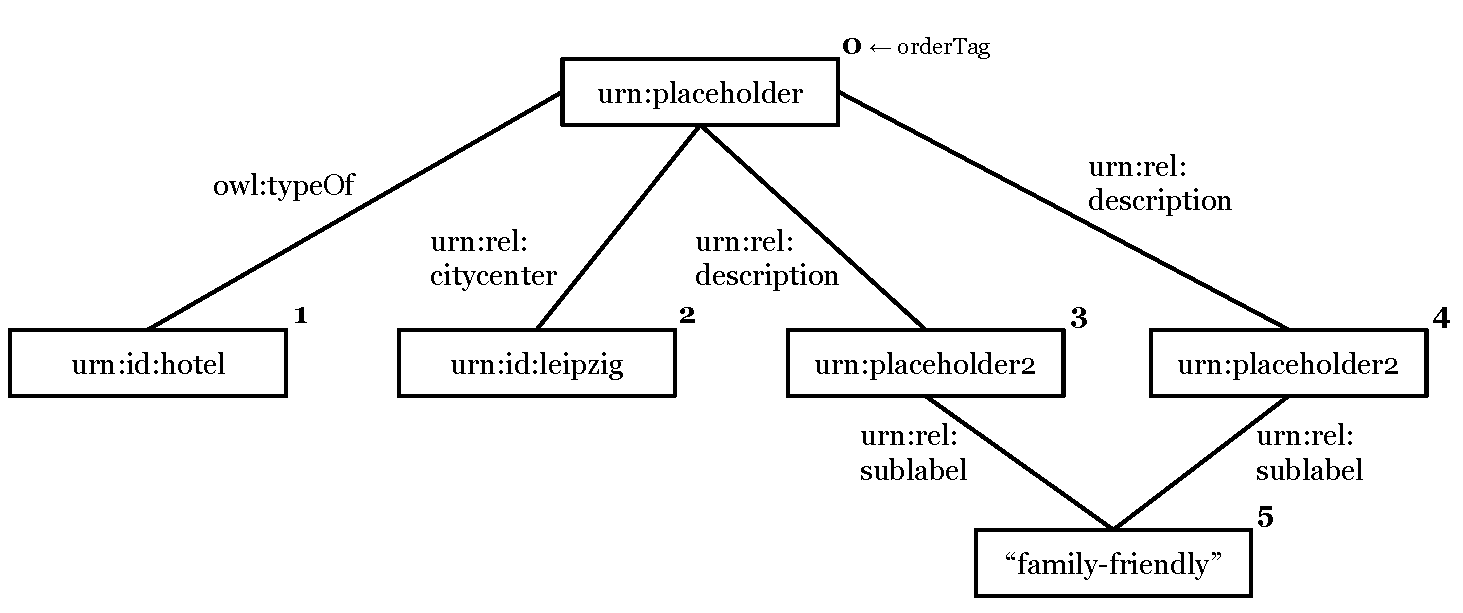
\includegraphics[width=\textwidth]{part_03/SEMANTiCS_architecture/query_plan_tree.pdf}
\caption{Scheduled query plan after topological sorting.}
\label{queryplantree}
\end{figure}



This definition satisfies Requirement \ref{req:allrelevantparts}.
Imagine a user wants to pose the following query to our framework: 
\begin{ex}
family-friendly hotel in Leipzig
\end{ex}

The annotated example query is shown in Figure~\ref{fig:ex2}.
In this example, \ssfulltext\ is an IRI of a service providing a full text search, \sstriplestore\ references a triple store and \ssgeo\ points to a search service encapsulating a GIS server.


\section{Search Query Interpretation}\label{chafedsearch:sec:queryinterpretation}

\todo[inline]{I don't get the following section at all! From the requirement that a query has to be interpreted by at least one service, how can we conlcude (``hence'') that the query plan is a topologically ordered graph with the result as root node? Maybe provide an example for clarity!? --Max}

Given a structured and annotated search query, a rea\-so\-nable query plan for the eligible search services has to be computed.
This can be done by scheduling algorithms with different optimization strategies. 
In this paper, we will focus on the general requirements only.

\todo[inline]{There is only one requirement, isn't there? So why focus on the ``general requirement\textbf{s}''? --Max}

\begin{req}
All triples of a structured and annotated search query have to be interpreted by at least one search service.
\end{req}
Note: As mentioned before, it is explicitly possible to have a triple interpreted by more than one search service.

Hence, a query plan can be computed by creating a to\-po\-lo\-gi\-cal order \cite{DBLP:books/aw/Knuth81}\ of the graph defined by the triples (\ie the triple S\,P\,O is interpreted as $S \xrightarrow{P} O$) of the structured search query where the result node is the root node of the graph.
A straight-forward implementation is shown in Fi\-gure \ref{fig:scheduler}.
There is numerous existing work dedicated to scheduler implementations \cite{XXX,YYY,ZZZ}.
A schedule graph is shown in Figure \ref{queryplantree} with respect to our running example.
\todo[inline]{Wo soll das Bild hin? Beschreibung?}


\section{Federated Search Architecture}\label{chafedsearch:sec:federated}

In this section, we present our federated search in\-fra\-struc\-ture. 
Particularly, it contains a service layer to which the diverse search services can be connected. 

\subsection{Search Service Interface}
For integration into the overall system, all search services have to implement a specific interface that facilitates exchangeability.
As a consequence, by implementing this given interface, services can be loosely coupled to the service layer.
The search service interface is defined as follows:
%\begin{figure}[h!tb]
\begin{lstlisting}[language=Java]
interface SearchService {
    /* annotation
     * in: search query Q
     * out: annotated search query A
     */ 
    A annotateQuery(Q);
    
    /* query execution 
     * in: annotated search query A
     * out: search results R
     */
    R executeQuery(A);
}
\end{lstlisting}
%\end{figure}
It is common to call \code{annotateQuery}\ with a complete structured query \code{Q}\ to get a complete annotated query \code{A}\ of all triples contained in \code{Q}.
Yet, the \code{executeQuery}\ method of an implementing search service is usually called passing only the sub-query the service is eligible for (\eg passing only the property \texttt{in Leipzig} to the geospatial search service).
Eligibility of a service is decided by the scheduler.

\subsection{Search Provider}
%The search provider provides an interface for search services that have implemented the search service interface.
%The definition of its interface is straight forward.
The search provider is an interface for integrated search services and defined as follows:
%\begin{figure}[h!tb]
\begin{lstlisting}[language=Java]
interface SearchProvider {
    /* query execution 
     * in: search query Q
     * out: search results R
     */
    R executeQuery(Q);
    
    /* search service registration 
     * in: IRI of the search service
     */
    void register(IRI);
    
    /* deregister a search service  
     * in: IRI of the search service
     */
    void deregister(IRI);
}
\end{lstlisting}
%\end{figure}
Hence, the search provider provides a method (\code{executeQuery}) for been accessed from a client while it also works as directory server (similar to a UDDI server \cite{UDDI}).
The directory functionality is achieved by the \code{register}\ and \code{deregister}\ methods allowing search services to connect and disconnect from the search provider.


%\subsection{Properties of the Architecture}
%The presented architecture separates different search functionality. 
%It decouples the search services from each other and  and allows an independent development, maintaince and 


% \subsection{Cache Layer}





\section{Conclusions}\label{chafedsearch:sec:conclusion}

We presented an architecture for a distributed search following the principles of service-oriented architectures. 
For this, we introduced a descriptive data representation, \ie the data representation does not contain implementation details of the underlying search services. 
Our implementation of such a structured search query is based on RDF.
After the tagging process, the annotated structured search query can be expressed using our RDF-like representation only.%, although, such a RDF representation will be very voluminous.
%However, we consider this as implementation detail. 

Our main contribution is the proposed architecture's capability of integrating and disintegrating (RDF unaware) search services dynamically.
This property is achieved by the descriptive message format as well as the ge\-ne\-ra\-lized service interface, which allows for a stateless and transparent communication with the integrated search services.
Hence, completely novel use cases are possible, in which search service integration happens on-the-fly to facilitate more dynamic environments.
Since the architecture is agnostic to the functionality of the search services, it is possible to integrate search services having not only (RDF-driven) semantic search functionalities but also other specialized search capabilities. 
For example, search services could comprise any specialized search functionality like ElasticSearch (providing high-performance federated large-scale full text search), or Web APIs encapsulating search functions with special semantics like SoundCloud\footnote{https://developers.soundcloud.com/}\ or Github\footnote{https://developer.github.com/}.
Our approach is superior as it does not burden these search services with the interpretation of the complete RDF (or SPARQL) standard.
Moreover, the architecture is scalable by design in the sense of the capability of integrating scalable and distributable search services. 
Finally, our \code{SearchProvider}\ provides a generalized interface being capable of receiving search queries via SPARQL (or any other representation, such as SQL or SeRQL). 
Therefore, a consolidated view on the dynamically summarized search services can be provided.
This allows for a transparent integration as a SPARQL endpoint, or using any other data access standard.

In the future, we will evaluate the capabilities of our architecture of providing rapid access to distributed data resources by comparing an implementation of the architecture to monolithic approaches. 
As possible data resources we consider datasets of the Linked Open Data Cloud as well as unstructured data provided by the Document Web in general or private data sets with restricted accessibility (by account or on the network level).
Hence, providing per\-so\-na\-lized search functionalities seems to be achievable.

Finally, the implementations are yet to be evaluated regarding performance and (re-)ranking issues. 
In the context of providing a distributed search, these are the main challenges considering the user's demands w.r.t.\ usability.

% However, increasing implementation details can lead to reducing the extendability with respect to search services which are not native to SPARQL.

%---

%Crucial for architecture -> rapid annotation has to be possible

%Requirements of the search queries w.r.t. SOA

%Evaluate the query plans with overlapping triple evaluation.

%Future:
%- sublabel
%- tighter integration
%- independent from the database of the search services 



%\bibliographystyle{abbrv}
%\bibliography{sigproc,refs} 
%\end{document}